\section{Data and simulated samples}\label{chap5:dataset}

This analysis makes use of data recorded in proton-proton collisions at 13\TeV during 2015, corresponding to a total integrated luminosity of 2.3\ifb. Events are selected according to single and double lepton triggers, similarly to the 8\TeV analysis. The HLT trigger \pt thresholds used in this analysis are listed in Table~\ref{tab:trigger13TeV}. Trigger efficiencies are measured in data and applied to simulated events as described in Sec.~\ref{sec:trigeff}.

\begin{table}[htb]
\begin{center}
\caption{Transverse momentum thresholds required for lepton triggers at HLT level. 
         Double set of thresholds indicates the thresholds for each leg of the double lepton triggers.}
\begin{tabular}{ccc}
\toprule
Trigger path       & Threshold \\
\midrule
Single electron    & $\pt > 23$\GeV         \\  
Single muon        & $\pt > 20$\GeV         \\ 
Muon-Electron      & $\pt > 17$ and $12$\GeV         \\ 
Electron-Muon      & $\pt > 17$ and $8$\GeV         \\ 
\bottomrule
\end{tabular}
\label{tab:trigger13TeV} 
\end{center}
\end{table}

\begin{comment}
\begin{table}[h]
\caption{HLT paths related to Electrons}
\label{table:ele_trigg_13}
\scalebox{0.75}{
\begin{tabular}{ll}
\hline
HLT Path & Description \\
\hline\hline
HLT\_Ele23\_WPLoose\_Gsf\_v*   &
\parbox{11cm}{$\,$ \\Single Electron trigger. Best trigger to be used for 2015 data. In HWW, we are using ``Trigger safe'' Id. Turn on is at around Ele $\rm p_{T}$ = 30 GeV\\}\\
\hline
HLT\_Ele17\_Ele12\_CaloIdL\_TrackIdL\_IsoVL\_DZ\_v* &
\parbox{11cm}{$\,$ \\Double Electron Trigger. Best trigger to cover the turn on region from single electron trigger. ``DZ'' filter is also present. Its efficiency is also calculated separately.}\\
\hline
HLT\_Ele12\_CaloIdL\_TrackIdL\_IsoVL\_v* &
\parbox{11cm}{$\,$ \\This electron leg of \\
HLT\_Mu17\_TrkIsoVVL\_Ele12\_CaloIdL\_TrackIdL\_IsoVL\_v*\\
same as Ele12 leg of double electron trigger.\\} \\
\hline
HLT\_Ele17\_CaloIdL\_TrackIdL\_IsoVL\_v*&
\parbox{11cm}{$\,$ \\This electron leg of\\
HLT\_Mu8\_TrkIsoVVL\_Ele17\_CaloIdL\_TrackIdL\_IsoVL\_v* \\
same as Ele17 leg of double electron trigger.} \\
\hline
\end{tabular}
}
\end{table}

\begin{table}
\caption{Muon trigger's elements description}
\label{table:mu_trigg_13}
\scalebox{0.8}{
\begin{tabular}{ll}
\hline
HLT path \\
\hline\hline
HLT\_IsoMu18\_v*   & 
\parbox{11cm}{$\,$ \\single muon trigger\\}\\
\hline
HLT\_IsoTrMu20\_v* &
\parbox{11cm}{$\,$ \\single muon trigger with tracker isolation\\}\\
\hline
HLT\_Mu17\_TrkIsoVVL & 
\parbox{11cm}{$\,$ \\leg for the HLT\_Mu17\_TrkIsoVVL\_Mu8\_TrkIsoVVL\_DZ\_v*,\\
HLT\_Mu17\_TrkIsoVVL\_TkMu8\_TrkIsoVVL\_DZ\_v* and\\ 
HLT\_Mu17\_TrkIsoVVL\_Ele12\_CaloIdL\_TrackIdL\_IsoVL\_v*\\
double lepton triggers\\} \\
\hline
HLT\_Mu8\_TrkIsoVVL &
\parbox{11cm}{$\,$ \\leg for the HLT\_Mu17\_TrkIsoVVL\_Mu8\_TrkIsoVVL\_DZ\_v* and\\
HLT\_Mu8\_TrkIsoVVL\_Ele17\_CaloIdL\_TrackIdL\_IsoVL\_v* \\ 
double lepton triggers\\} \\
\hline
HLT\_TkMu8\_TrkIsoVVL &
\parbox{11cm}{$\,$ \\leg for the HLT\_Mu17\_TrkIsoVVL\_TkMu8\_TrkIsoVVL\_DZ\_v*\\
double muon trigger\\} \\
\hline
$DZ_{\mu\mu}$ &
\parbox{11cm}{$\,$ \\efficiency of DZ cut in \\
the HLT\_Mu17\_TrkIsoVVL\_Mu8\_TrkIsoVVL\_DZ\_v*\\
and HLT\_Mu17\_TrkIsoVVL\_TkMu8\_TrkIsoVVL\_DZ\_v* \\
double muon triggers, it is around 95\%\\} \\
\hline
\end{tabular}
}
\end{table}
\end{comment}


%Monte Carlo
Concerning the simulated samples, several different MC generators are used. 
Higgs boson signal samples are simulated using \textsc{Powheg v2}~\cite{Nason:2004rx,Frixione:2007vw,Alioli:2010xd}, designed to generate these processes with NLO QCD accuracy.
In particular, for Higgs boson produced via ggH~\cite{Alioli:2008tz} and VBF~\cite{Nason:2009ai},
the decay into two W bosons and subsequently into leptons is done using \textsc{JHUGen} v5.2.5. 
For associated production with a vector boson ($\mathrm{W}^{+}\mathrm{H}$, $\mathrm{W}^{-}\mathrm{H}$, ZH)~\cite{Luisoni:2013kna}, including gluon fusion produced ZH (ggZH), 
the Higgs boson decay is instead simulated using \textsc{pythia} 8.1~\cite{Sjostrand:2007gs}. All the signal samples are generated assuming a Higgs boson mass of 125\GeV.

The \textsc{Powheg v2}~\cite{Melia:2011tj} is also used for simulating the $\mathrm{q\bar q}$ induced WW  production in different decay channels. The simulated events are reweighted to reproduce the $\pt^\mathrm{WW}$ distribution obtained from \pt-resummed calculations~\cite{Meade:2014fca,Jaiswal:2014yba}. Gluon fusion produced WW is generated at LO QCD accuracy using \textsc{mcfm} v7.0~\cite{Campbell:2013wga}.
%The cross section used for normalizing WW processes produced via $\mathrm{q\bar q}$ was computed at next-to-next-to-leading order (NNLO)~\cite{Gehrmann:2014fva}. 
%In order to control the top quark background processes, the analysis is performed with events that have no more than one high-\pt jet. The veto on high-\pt jets enhances the importance of logarithms of the jet \pt, spoiling the convergence of fixed-order calculations of the qq$\rightarrow$WW process and requiring the use of dedicated resummation techniques for an accurate prediction of differential distributions~\cite{Meade:2014fca,Jaiswal:2014yba}. The \pt of the jets produced in association with the WW system is strongly correlated with its transverse momentum, $\pt^\mathrm{WW}$, especially in the case where only one jet is produced. The simulated qq$\rightarrow$WW events are reweighted to reproduce the $\pt^\mathrm{WW}$ distribution from the \pt-resummed calculation.

The \ttbar process with dilepton final state is also generated using \textsc{Powheg v2}. The simulated processes for the WW and \ttbar production are illustrated in Table~\ref{tab:wwl}, together with the associated cross sections. Other minor background samples are also generated, a list of the most relevant ones is presented in Table~\ref{tab:otherbck}.

\begin{table}[htb]
\caption{Simulated processes for \ttbar and \WW production.}\label{tab:wwl}
\begin{center}
\begin{tabular}{lc}
\toprule
Process & $\sigma\times\mathcal{B}$ [pb] \\
\midrule
\ttbar$\rightarrow$WW$\mathrm{b\bar{b}}\rightarrow2\ell2\nu \mathrm{b\bar{b}}$ & 87.31 \\
$\mathrm{q\bar q}\rightarrow$WW$\rightarrow2\ell2\nu$ & 12.178 \\
$\mathrm{gg}\rightarrow$WW$\rightarrow2\ell2\nu$ & 0.5905 \\
%$gg\rightarrow$\WW$\rightarrow2\ell2\nu$ (H diagr.) & 0.9544\\
\bottomrule
\end{tabular}
\end{center}
\end{table}

\begin{table}[htb]
\caption{Simulated samples for other minor background processes used in the analysis. Single top quark production includes the dominant tW process, as well as the sub-dominant production in the s- and t-channels.\label{tab:otherbck}}
\begin{center}
\begin{tabular}{lc}
\toprule
Process & $\sigma\times\mathcal{B}$ [pb] \\
\midrule
Drell-Yan ($10\GeV < \mll < 50\GeV$)  &  20471.0  \\
Drell-Yan ($\mll > 50\GeV$)   &  6025.26  \\
Single top &   71.7  \\
WZ$\to2\ell2\mathrm{q}$ &  5.5950 \\
ZZ$\to2\ell2\mathrm{q}$ &  3.2210 \\
WWZ &  0.1651 \\
WZZ &  0.05565 \\
ZZZ &  0.01398  \\
\bottomrule
\end{tabular}
\end{center}
\end{table}

All processes are generated using NNPDF2.3~\cite{Ball:2013hta,Ball:2011uy} for NLO generators.
The LO version of the same PDF set is used for LO generators. All the event generators are interfaced  to \textsc{pythia} 8.1~\cite{Sjostrand:2007gs} for the showering of
partons and hadronization, as well as for including a simulation of underlying event (UE) and multiple parton interaction (MPI) based on the CUET8PM1 tune~\cite{Khachatryan:2015pea}. 

To estimate the systematic uncertainties related to the choice of UE and MPI tunes, the signal processes and the WW background are generated with two alternative tunes which are representative of the errors on the tuning parameters.
The showering and hadronization systematic uncertainty is estimated by interfacing the same MC samples with the \textsc{herwig++} 2.7 parton shower~\cite{Richardson:2013nfo,Bellm:2013hwb} instead of \textsc{pythia 8}.

Drell-Yan (DY) production of Z/$\gamma^{*}$ is generated using \textsc{amc@nlo}~\cite{Alwall:2014hca}. 
Other multiboson processes, such as WZ, ZZ, and VVV (V$=$W/Z), are generated with \textsc{amc@nlo} and normalized to the cross section calculated at NLO accuracy.

The simulated samples are generated with distributions for the number of pile-up interactions that are meant to roughly cover, though not exactly match, the conditions expected for the different data taking periods. In order to factorize these effects, the number of true pile-up interactions from the simulation truth is reweighted to match the data.
In Fig.~\ref{Fig:pu}, the effect of this reweighting on a sample enriched in Drell-Yan events is shown. The average number of pile-up is approximately $11.5$.

\begin{figure}[htbp]
\centering
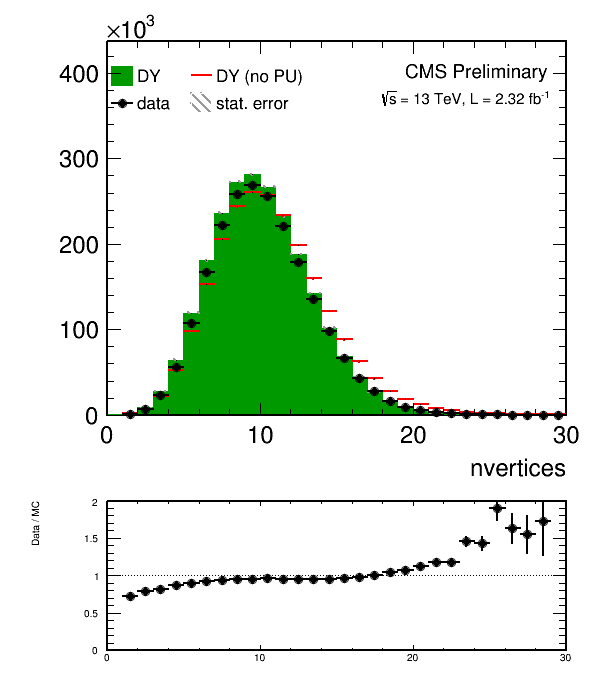
\includegraphics[width=0.45\textwidth]{images/13TeV/nvertices.png}
\caption{
    Distribution of the number of vertices in a Drell-Yan enriched phase space in data,
    together with the simulation before (red) and after (solid green) the pile-up reweighting.}
    \label{Fig:pu}
\end{figure}

For Higgs boson signal, the inclusive cross sections used are the ones reported by the LHC Higgs Cross Section Working Group~\cite{temphiggsxsecs}. The ggH cross section is computed at NNLO+NNLL QCD and NLO EW accuracy, while NNLO QCD and NLO EW accuracy is used for the other production modes. The branching fractions are the ones reported in Ref.~\cite{Heinemeyer:2013tqa}.

The cross section used for the $\mathrm{q\bar q}$ induced WW processes is computed at NNLO QCD accuracy~\cite{Gehrmann:2014fva}. The normalization of this background is eventually directly taken from a fit to data and the NNLO cross section is used as initial guess. The LO cross section for the gluon induced WW process is obtained directly from \textsc{mcfm}, and a $k$-factor of 1.4 is applied to correct for the difference between the LO and NLO theoretical calculation~\cite{Caola:2015rqy}.
The contribution of the interference between the $\mathrm{gg \to WW}$ and $\mathrm{gg\to H\to WW}$ processes is evaluated using \textsc{mcfm} and is found to be negligible compared to the signal contribution.

The cross sections of the different single top processes are estimated by the LHC Top Working group~\cite{singletop} with NLO accuracy.
The \ttbar cross section is also provided by the LHC Top Working group~\cite{topxsec}, and it is computed at NNLO QCD accuracy and NNLL accuracy for soft gluon resummation effects.

